\Chapter{Data Processing and Low-level Calibration}
\label{Ch7}

The purpose of detector calibration is to convert the raw DAQ signal output to event information with physical meaning.
The raw output of the from CAEN digitizers of the DAQ system is in binary format.
To convert the DAQ signal output to calibrated data, multiple procedures of data processing, shown in Figure~\ref{fig:Unpacking}, are required.
\begin{figure}[ht]
\centering
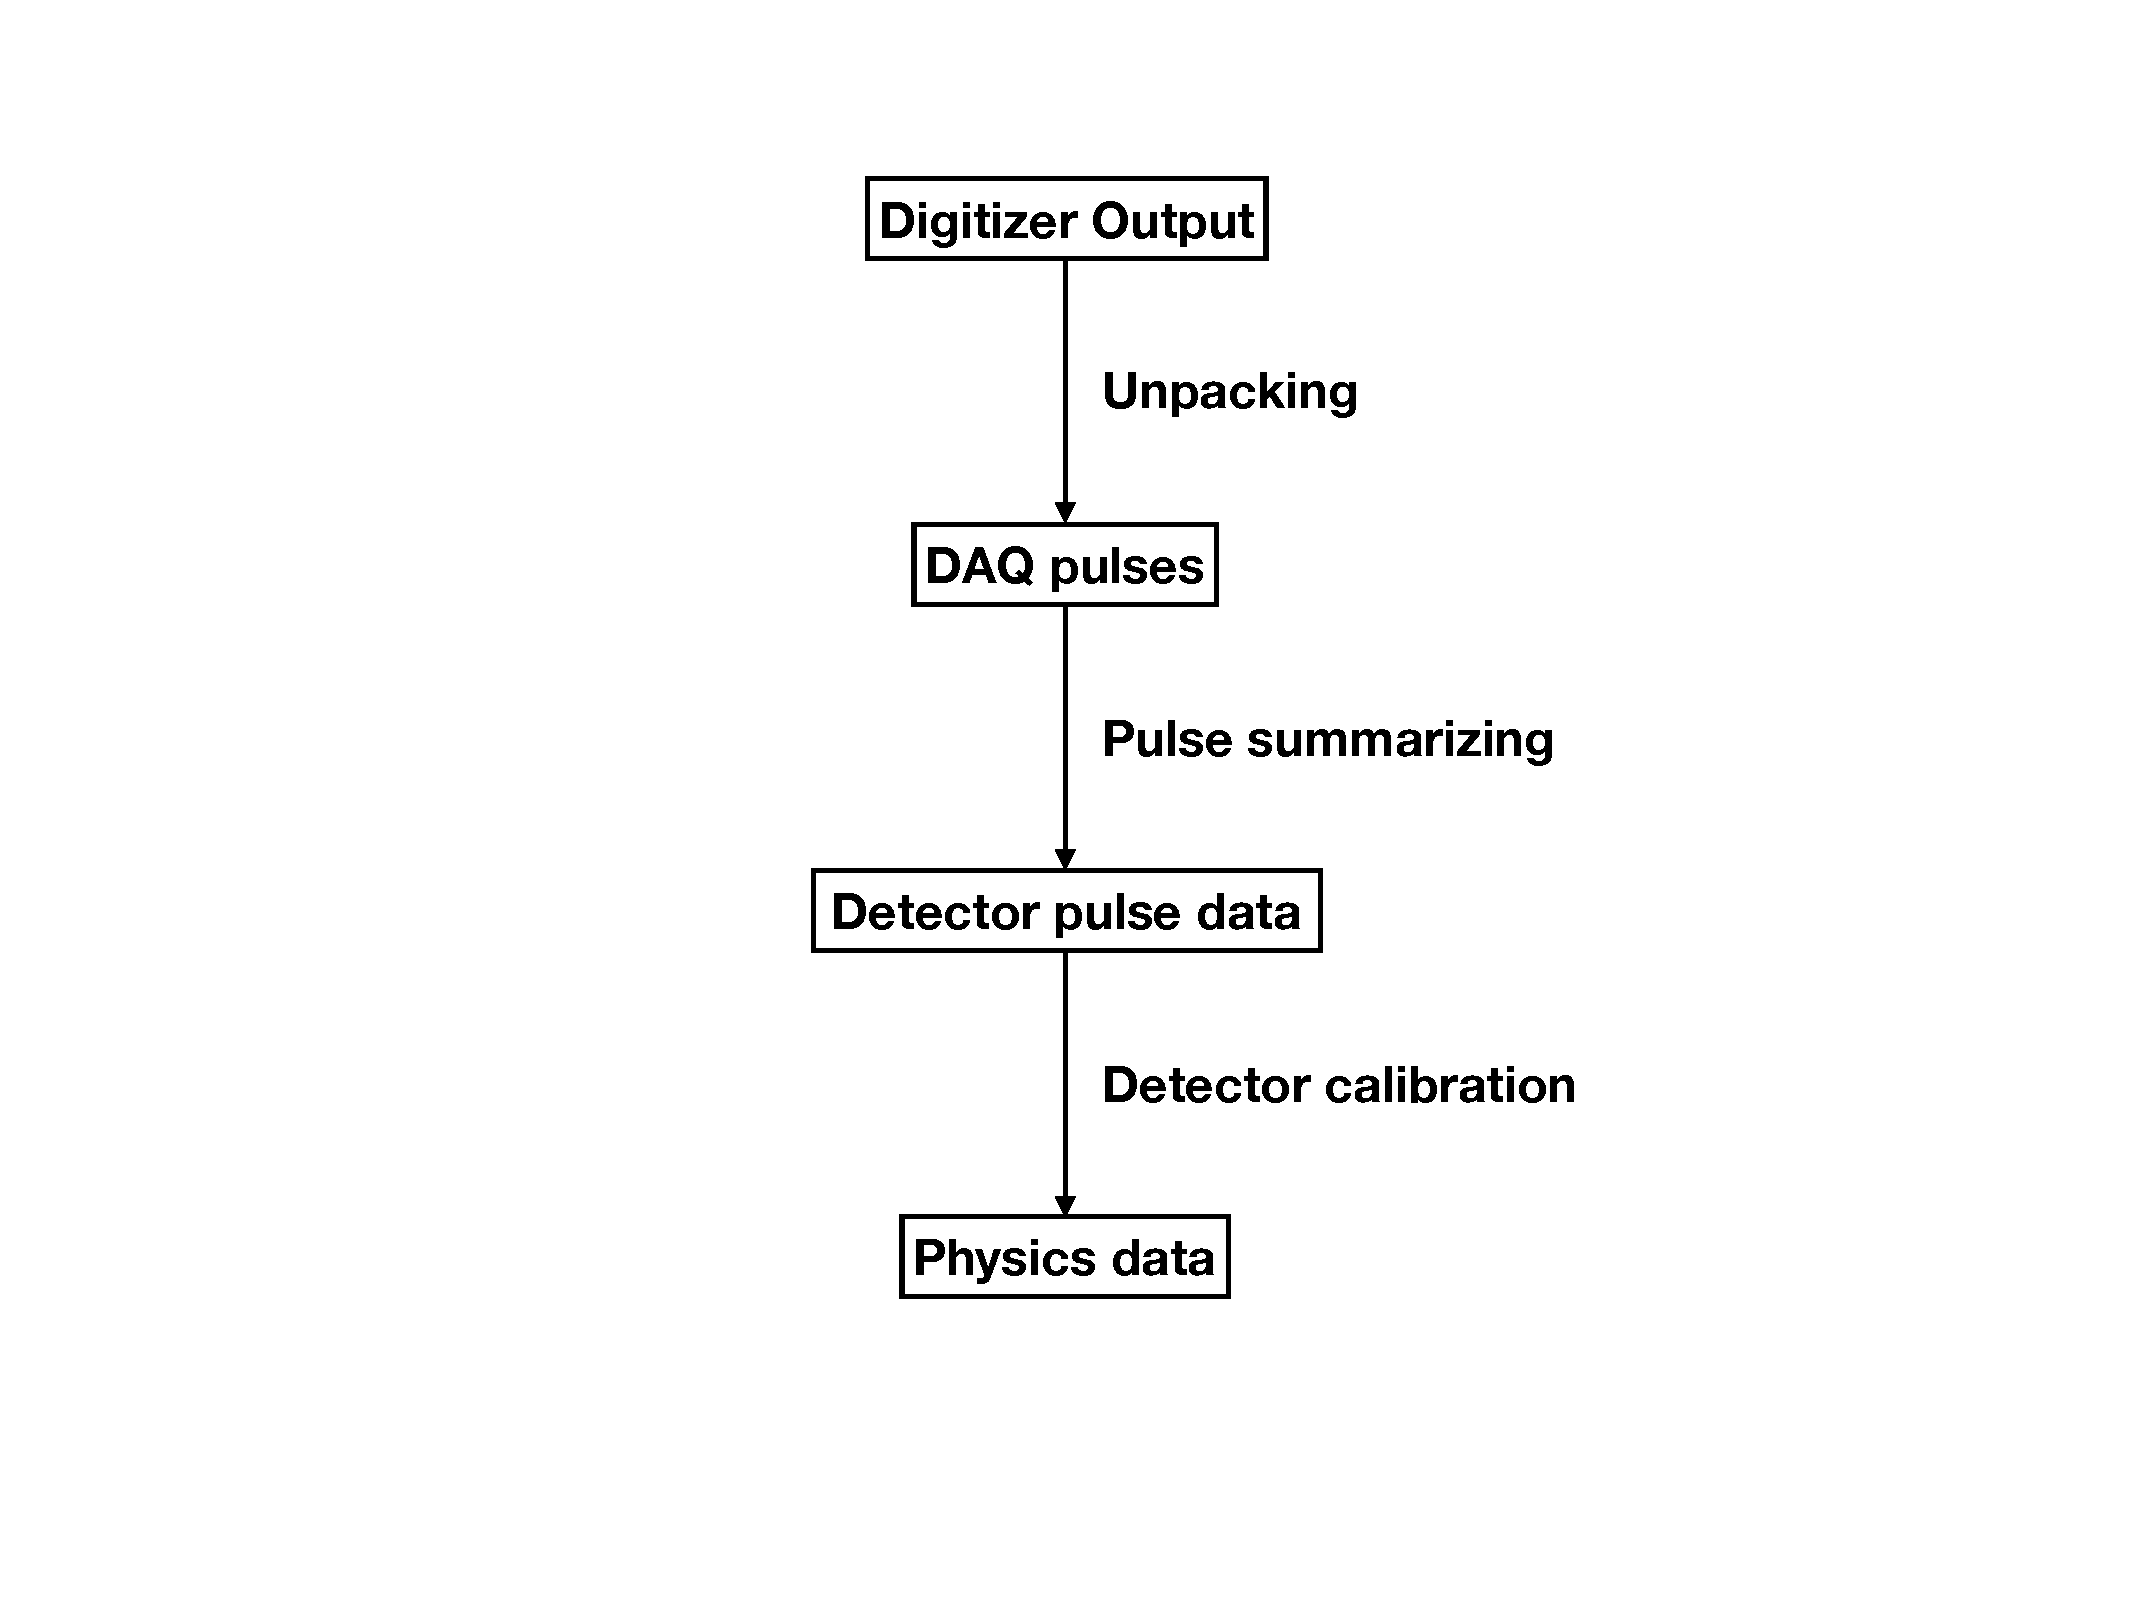
\includegraphics[width=0.9\textwidth]{Figures/DataUnpacking.pdf}
\caption[Data process procedures]{
Schematic of the data process procedures. 
}
\label{fig:Unpacking}
\end{figure}

\Section{Data Processing}

The raw output from the digitizers are unpacked from the binary format data of each DAQ channel to actual pulses collected by each channel.
The information saved after unpacking includes the absolute time of each sample, the event number assigned to a group of pulses close in time, the channel number and the values of all ADC samples in a pulse.
The unpack procedure contains minimum data analysis, merely converting the digitizer output to human-readable format.

The unpacked data saves all samples of every pulse and requires substantial disk space.
Summarizing the unpacked pulse data is necessary for the ease of accessing the data.
In the pulse summarizing procedure, each pulse's height, integral, absolute time, channel number and PSD value are saved.
The summarized values are the key variables used in event reconstruction, including time, reconstructed position, and reconstructed energy.

\Section{Timing Calibration}

A particles energy deposition, detected by both PMTs of a segment, is referred as a \textit{hit}.
A group of hits close in time is defined as a \textit{cluster} detected by the PROSPECT AD. 
In addition, many of the particle interactions in the PROSPECT AD, including IBD, are identified by time coincidences between clusters.
The position reconstruction of each hit relies on accurate timing difference between two PMTs.

\Subsection{Time Reconstruction}
Because the sampling rate of the digitizers are 250~MHz, the time difference between two samples is 4~ns.
The reconstructed time of each pulse is the interpolated timing of the half-height of the leading edge shown in Figure~\ref{fig:PulseTiming}.
\begin{figure}[ht]
\centering
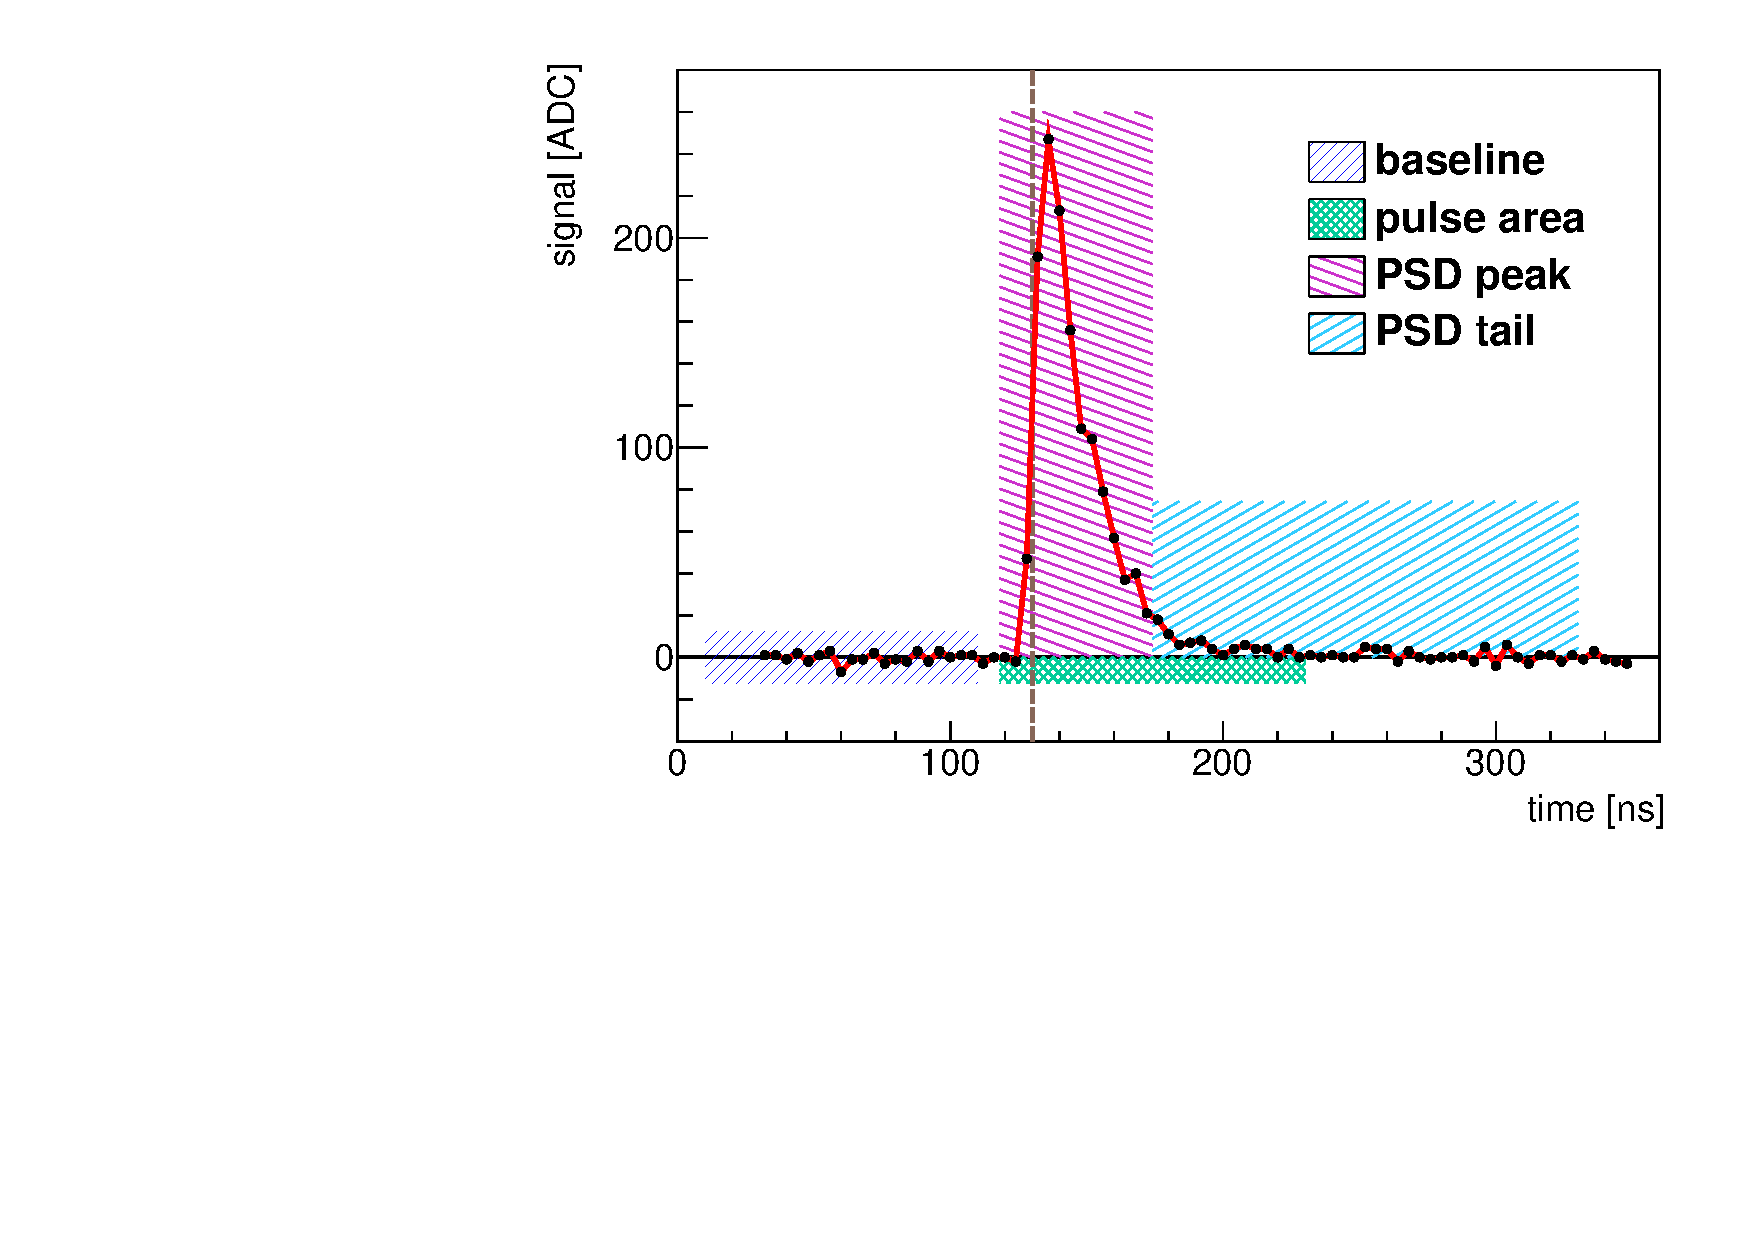
\includegraphics[width=0.6\textwidth]{Figures/PulseTiming.pdf}
\caption[Pulse timing reconstruction]{
An example pulse of PROSPECT. 
The rise-up timing of a pulse is defined as the time of the half-height leading edge of the pulse.
}
\label{fig:PulseTiming}
\end{figure}	

The reconstructed hit time is the rise-up time of the first pulse detected in a segment.
The beginning time of a cluster is the time of the hit with most scintillation light.

\Subsection{Timing Offset in Each Segment}
The natural differences in PMT signal transportation causes various time offsets between channels.
The event timing difference observed by two PMTs of each segment needs to be corrected based on the measurement of time offsets.
Cosmic muon tracks are used to measure the time offset of each segment.
Through-going muons produce multiple time correlated pulses among PMTs at various distances from the origin of scintillation light.
Because the PROSPECT AD is particle track sensitive, the muon tracks can be selected by cuts requiring multiple segment hits ($>=4$ segments and within 0.4 $\times$ segment width difference) with specific PSD value and high energy deposition requirements. 
Upon the selection of a narrow track of single muon cluster, the segment ``corner-clipping" hits are tagged within the detector dynamic range of light collection.
The corner-clipping hits are muon energy depositions constrained in a small range to reject additional particle interactions.
The time difference $\Delta t$ of corner-clipping muon hits are calculated.
The $\Delta t$ distribution offset from $\Delta t=0$ is the time offset between the two PMTs in each segment.
The time offsets in all detector segments are shown in Figure~\ref{fig:TimeOffset}.
\begin{figure}[ht]
\centering
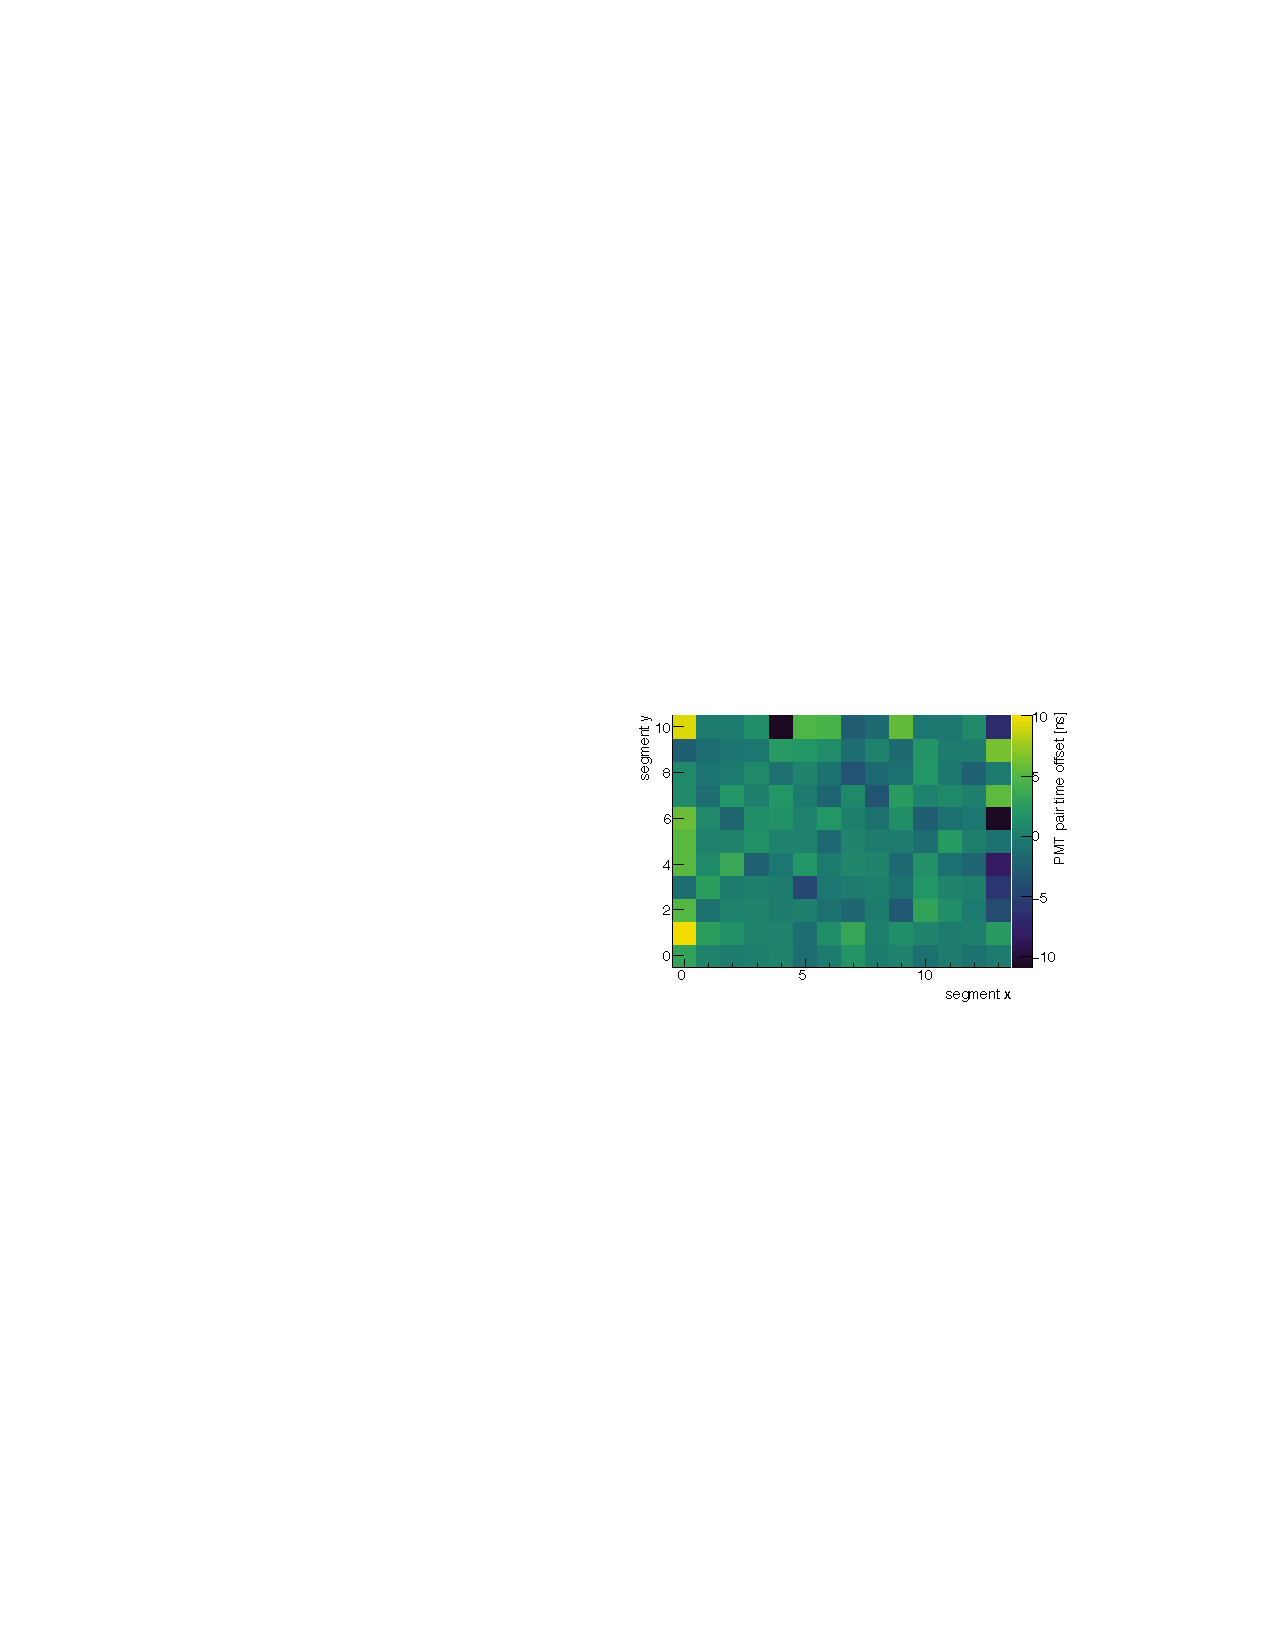
\includegraphics[width=0.8\textwidth]{Figures/TimeOffset.pdf}
\caption[Time offset in all detector segments]{
The time offset $\Delta t$ correction of all detector. 
The Hamamatsu PMTs indicate smaller time differences than the ET PMTs.
}
\label{fig:TimeOffset}
\end{figure}	

The OCS calibration is also used to demonstrate the time offset measured by the segment corner-clipping muon $\Delta t$ distribution, since all OCS light sources are ideally deployed at the center of each strung PLA rods. 
With both muon and OCS timing difference analysis, the run-to-run variation of time offset is $\sim$50~ps.

\Section{Position Calibration}

In Chapter~\ref{Ch4}, the horizontal and vertical segment locations were defined as $(x, y)$ positions of the reconstructed events.
For the baseline-dependent IBD measurement, the distance between the HFIR core and each segment can be converted from the $(x, y, z)$ position of segment hits.
The $(x, y, z)$ positions of hits are also use to select correlated events with respect to their distance.

The time difference between the PMTs of each segment is used to reconstruct a hit's position along the $z$-axis.
The PLA rod tabs, because of their precise widths and distances, make each PLA rod's axis good position calibration ``ruler".
By identifying light collection bands of the corner-clipping muon hits from muon tracks, the ``Hobbes effect" of muon energy deposition changed by the PLA tabs makes nonuniform event $dt$ distribution, as shown in Figure~\ref{fig:Tiger}.
\begin{figure}[ht]
\centering
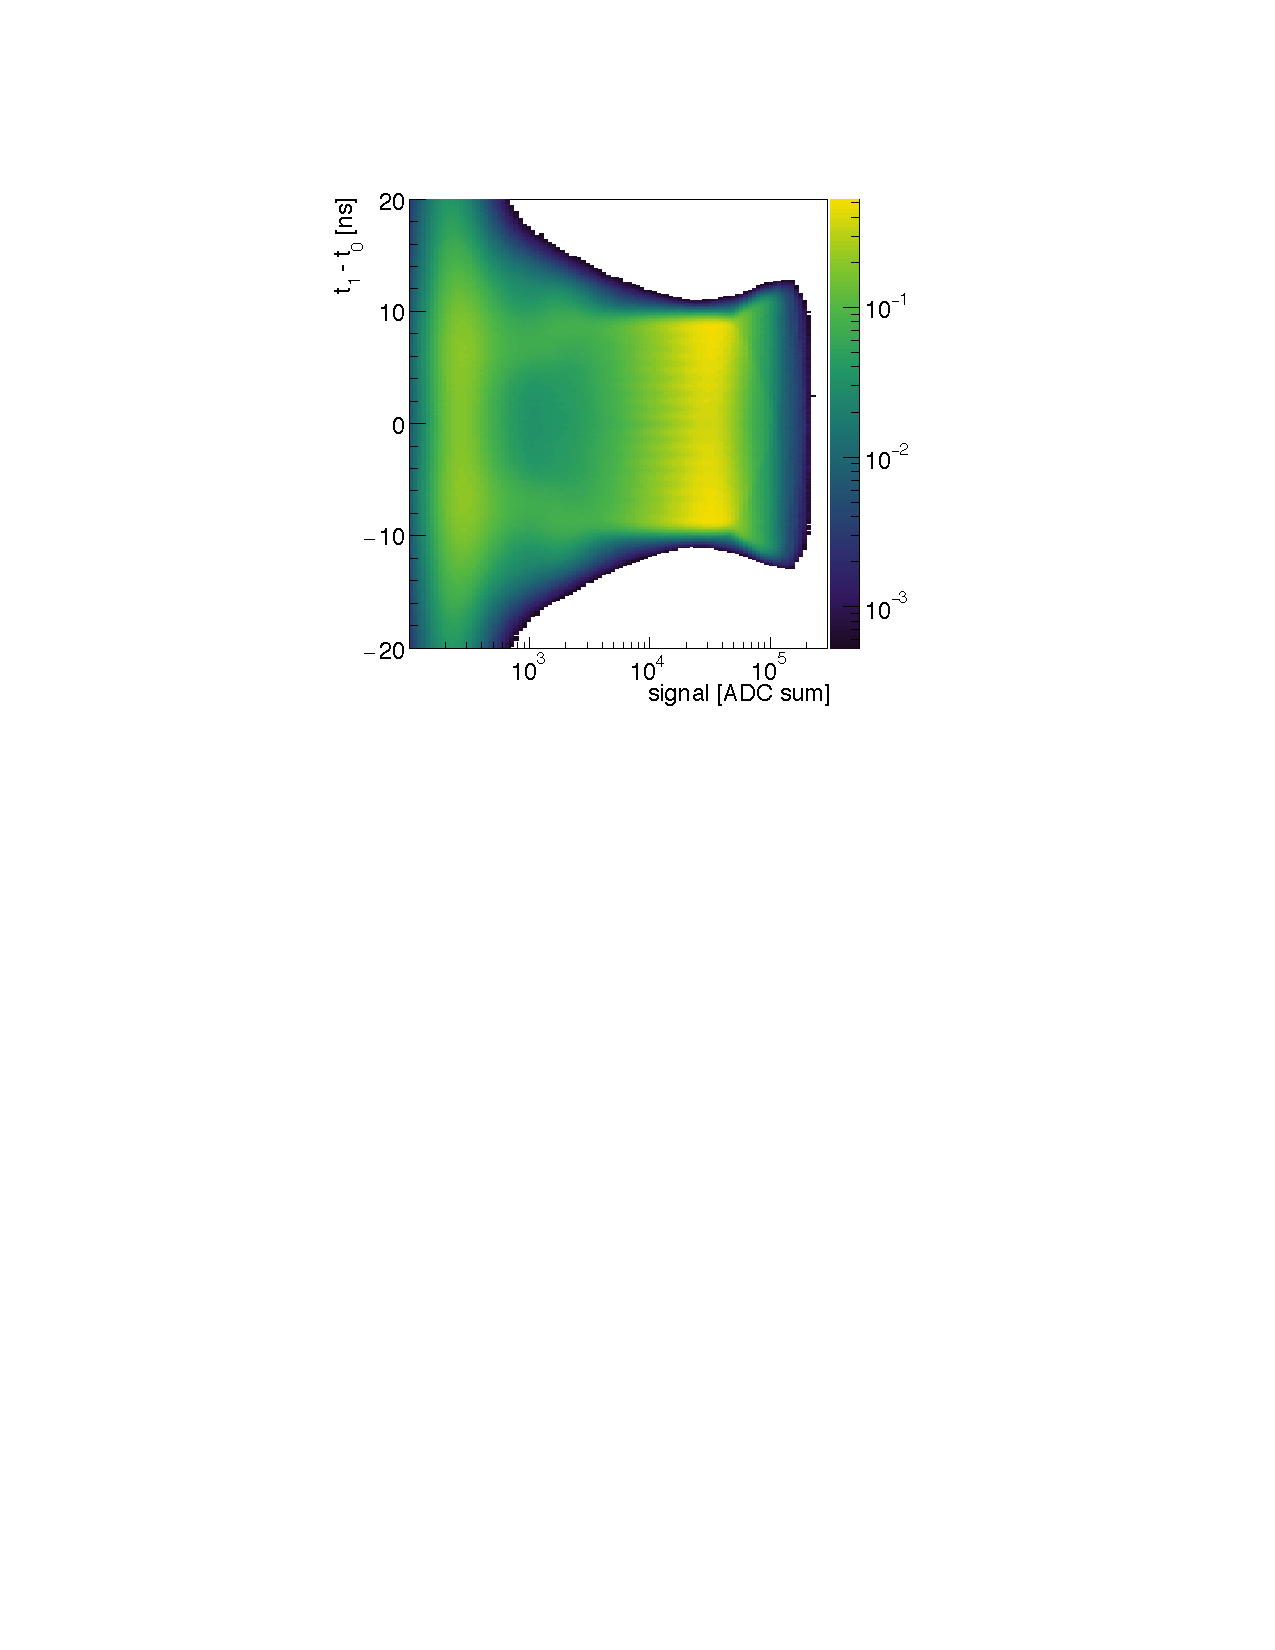
\includegraphics[width=0.6\textwidth]{Figures/TigerStrips.pdf}
\caption[The ``Hobbes effect” corner clipping muons]{
The ``Hobbes effect” corner clipping muons travel through different sections of a segment, where the $dt$ distribution varies with the existence of the PLA rods.
}
\label{fig:Tiger}
\end{figure}

The $dt$ distribution is fitted with a composite function shown in Figure~\ref{fig:TigerFit}.
\begin{equation}
f(dt) = M(dt)\left[1+k\cos(\frac{2\pi}{\delta}(a dt+b dt^3))\right],
\end{equation}
where $M(dt)$ is a ``M" shaped function, the fine structure contains the average $\delta$ = 78.5~mm  spacing between pinwheel tabs, and $k$, $a$, $b$ are fitting parameters.
Therefore, a $dt$ dependent $z(dt)$ reconstruction is expressed as
\begin{equation}
z(dt) = a dt+b dt^3.
\end{equation}
Scanning through the segments with calibration sources deployed at different $z$ position can also be used to calibrate the position reconstruction.
The result of scanning all segments with $^{137}$Cs single gammas demonstrated the effectiveness this strategy.
\begin{figure}[ht]
\centering
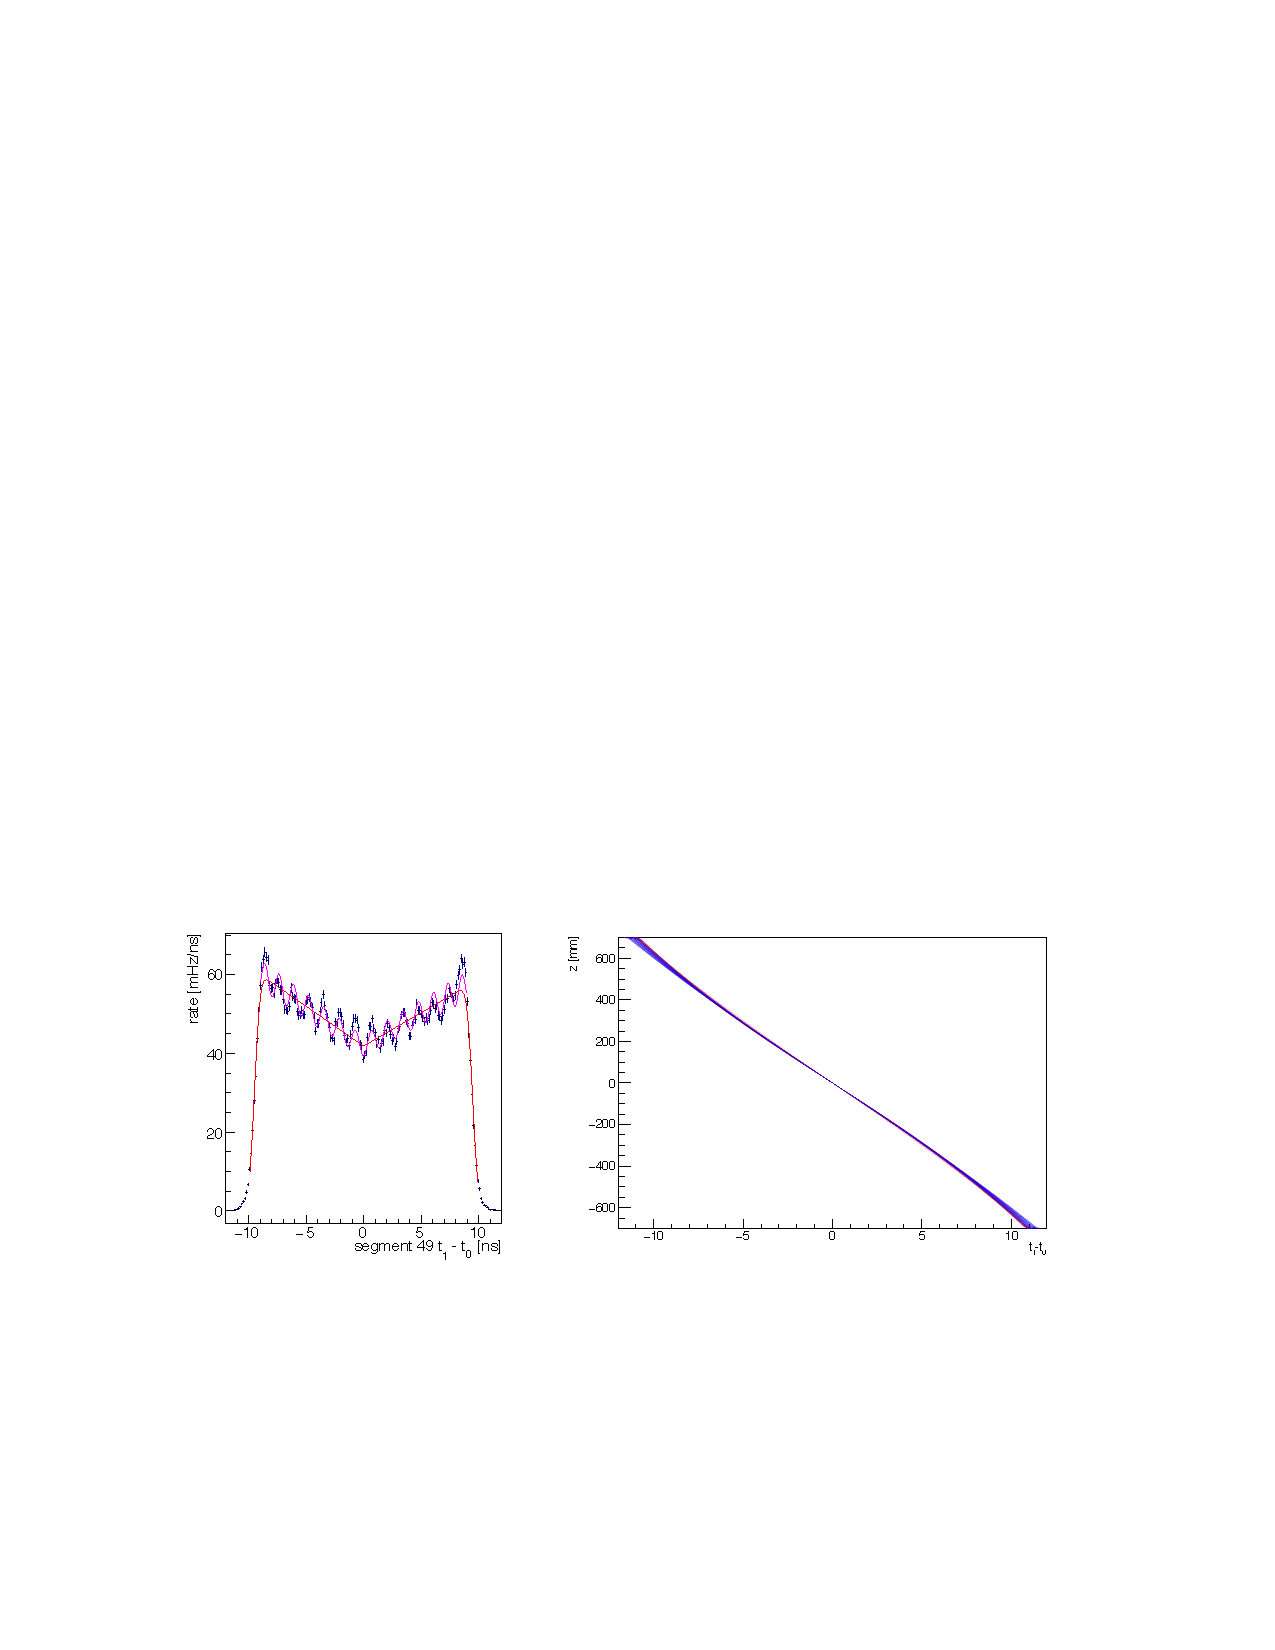
\includegraphics[width=0.95\textwidth]{Figures/TigerFit.pdf}
\caption[The fitted $z(dt)$ function]{
(Left) The fitted function of the $dt$ distribution.
(Right) The $z(dt)$ functions of all segments, where blue (red) represents segments with Hamamatsu (ET) PMTs.
}
\label{fig:TigerFit}
\end{figure}

\Section{ADC to Energy conversion}

Because the trigger and ZLE thresholds are higher than the SPE signal light collection, PROSPECT converts ADC integrals directly to reconstructed energy.
The calibration energy utilized for the ADC to energy conversion is the total visible energy of the $n$-Li capture events.
An advantage of calibrating the energy with $n$-Li events is their localized PSD and energy range.
The $n$-Li captures are selected based on time coincidence between proton recoils caused by fast cosmogenic neutrons and delayed hits in the PSD and energy range of $n$-Li captures.
Besides, muons and cosmogenic neutrons are constantly detected in the PROSPECT AD.
Passive energy calibration can be performed to ensure energy scale stability through the data acquisition period.
The total energy of a $n$-Li produced alpha particle and Triton is 4.78 MeV, which is severely quenched due to the particles' high $dE/dx$ rate.
The accurate quenched energy of $n$-Li capture event is unknown.
The initial ADC to energy conversion is hence based on an assumed energy of 0.55~MeV.
Further correction is made later as the absolute energy scale is calibrated separately through gamma sources and cosmogenic $^{12}$B calibrations.

The light collection of PMT channels decreases with increasing distance from the source of scintillation light.
This effect is due to the light attenuation and leakage when traveling through the scintillator in each segment.
To quantify the attenuation and correct the light collection of events with dependence on $z$ positions, two variables of a segment's light collection are defined as 
\begin{equation}
R(dt) = \frac{S_1}{S_0}; \	\ S(dt) = \sqrt{S_1S_0},
\end{equation}
where $S_1$ and $S_0$ are ADC integrals of two PMTs.
A relative light transport efficiency from a source to each PMT channels is defined as 
\begin{equation}
\eta_0(dt) = \frac{S(dt)\sqrt{R(dt)}}{S(0)\sqrt{R(0)}}; \	\  \eta_1(dt) = \frac{S(dt)\sqrt{R(0)}}{S(0)\sqrt{R(dt)}},
\end{equation}
where $dt = 0$ is defined as the time difference of a light source at the segment center.
The fitted light transport efficiency curve of all segments in the early data acquisition time period is shown in Figure~\ref{fig:EtaFit}.
\begin{figure}[ht]
\centering
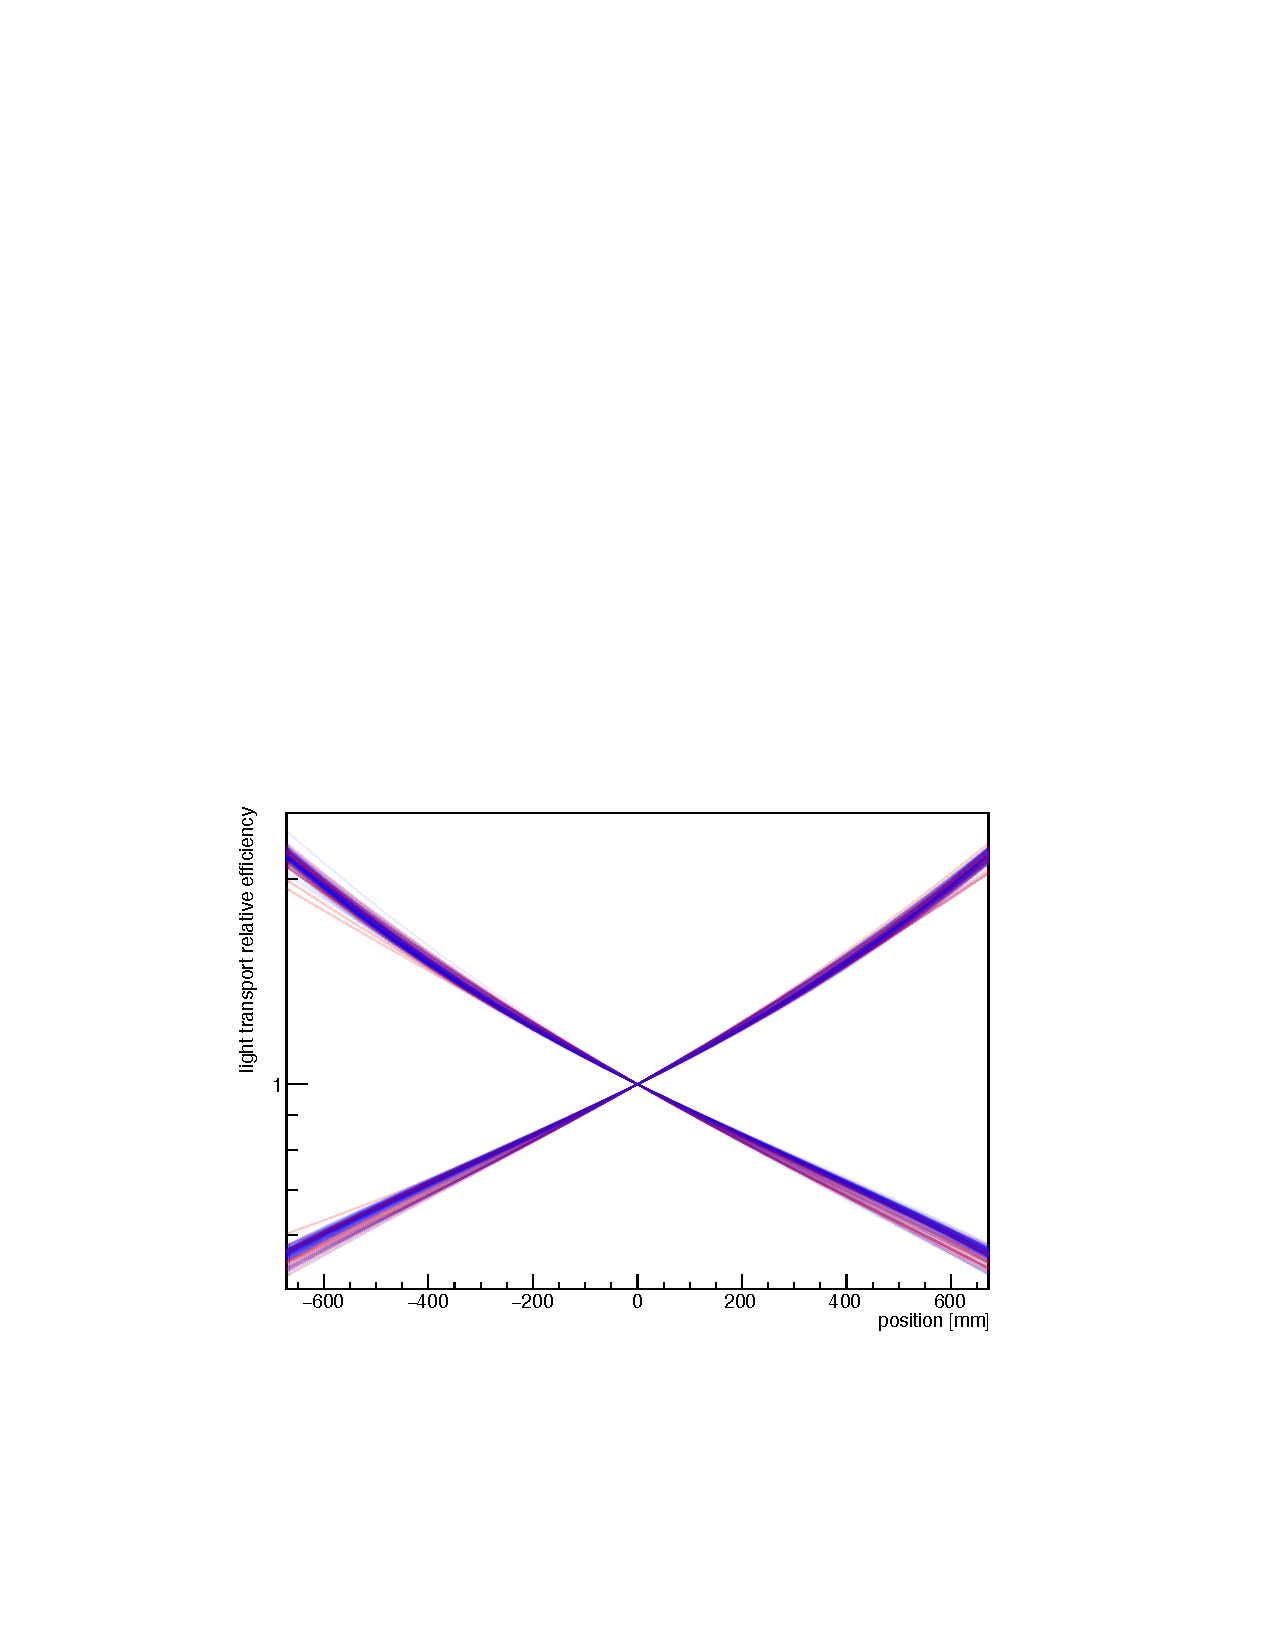
\includegraphics[width=0.8\textwidth]{Figures/EtaExpo.pdf}
\caption[The light transport efficiency curve of all segments]{
The light transport efficiency curve of all segments in log scale, where blue (red) curve represents Hamamatsu (ET) PMTs.
The curves show little deviations from exponential function.
}
\label{fig:EtaFit}
\end{figure}

The ln$(S_1/S_0)$ of each segment was found varying linearly with respect to $dt$, as shown in Figure~\ref{fig:lnR}.
The geometric mean is calculated with respect to $dt$, as shown in Figure~\ref{fig:GeoMean}.
The non-uniform ADC integral is corrected with the ADC to energy conversion factors
\begin{equation}
g_0 = \frac{S}{\sqrt{R}E_n}; \ 		\ g_1 = \frac{S\sqrt{R}}{E_n},
\end{equation}
where $E_n$ is the presumed $n$-Li visible energy.
These factors are unique for each channel at different times, ensuring consistent energy scale at all positions and times in the PROSPECT AD.
However, because of the inevitable variation of photo statistics at different location, the resolution of reconstructed energy needs further correction.
\begin{figure}[ht]
\centering
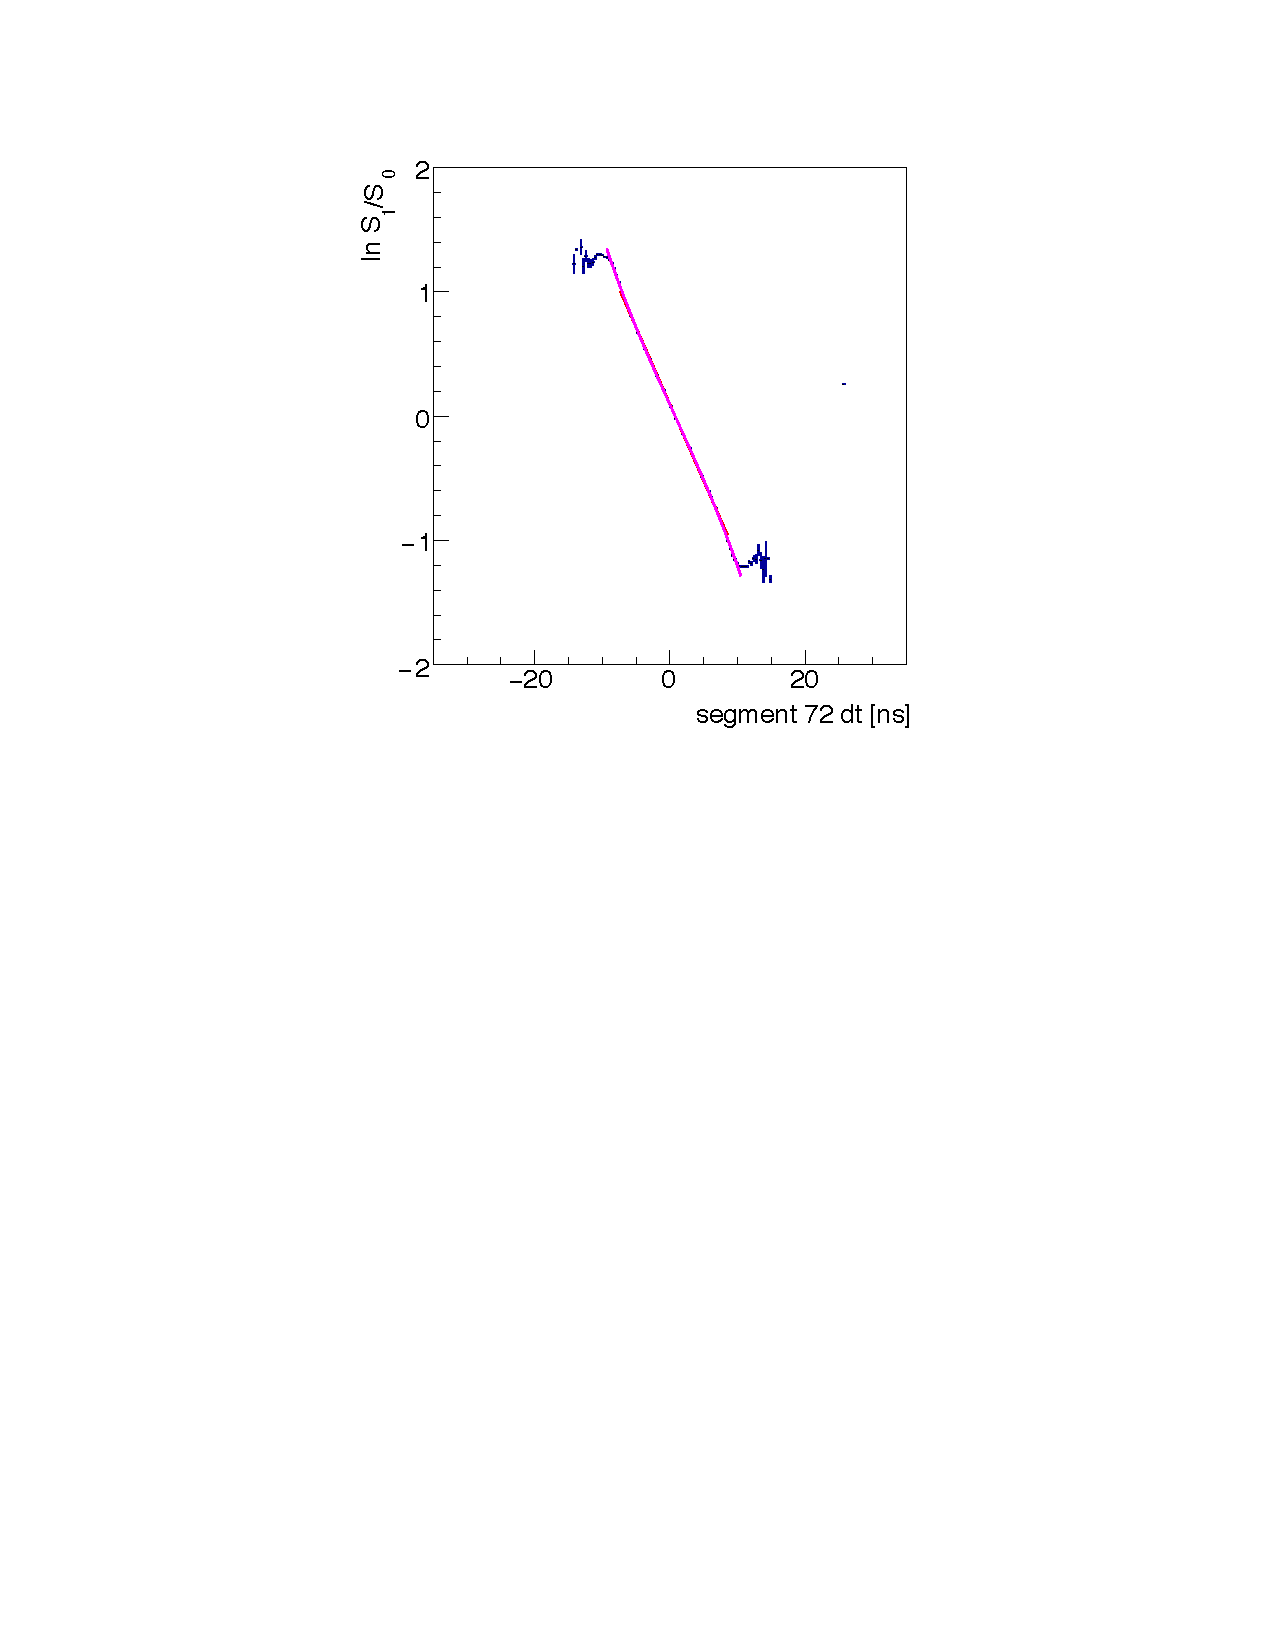
\includegraphics[width=0.6\textwidth]{Figures/lnRvsdt.pdf}
\caption[ln$(S_1/S_0)$ vs $dt$ of a segment ] {
The ln$(S_1/S_0)$ varies with respect to $dt$ of a randomly selected segment, where the red line is a linear fit; the pink line is the cubic polynomial used in this analysis.
}
\label{fig:lnR}
\end{figure}
\begin{figure}[h!]
\centering
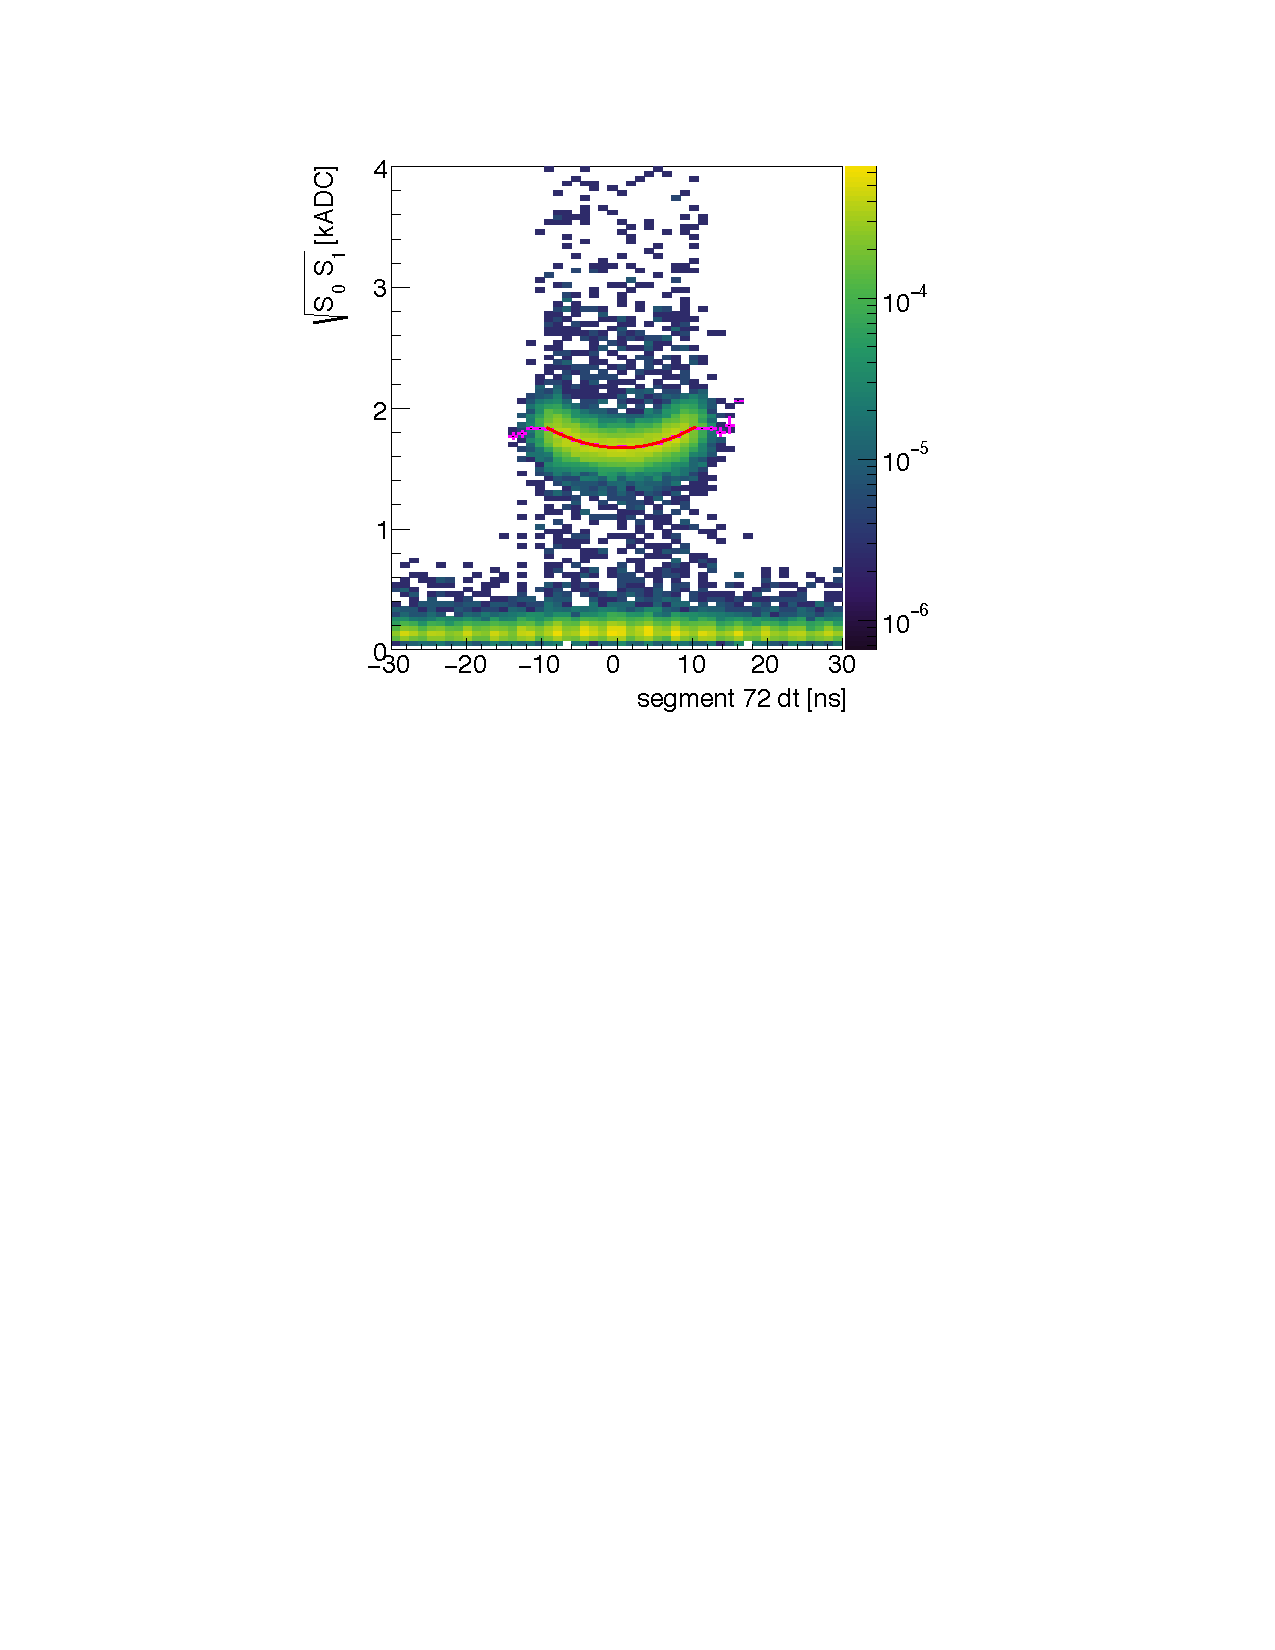
\includegraphics[width=0.6\textwidth]{Figures/GeometricMean.pdf}
\caption[The geometric mean of $n$-Li events ] {
The geometric mean of $n$-Li events are saved for each event with dependence on $dt$.
The total collected signal at the center of a segment is the minimum.
}
\label{fig:GeoMean}
\end{figure}

The SPE conversion between ADC and PE number was studied with OCS calibrations when the gain of each channel was set higher than the regular data taking configuration to cover single PE energy range.
By comparing the average ADC integrals of single PE and $n$-Li total energy, an MeV/PE photostatistic conversion can be made as shown in Figure~\ref{fig:SPE}
This photostatistical conversion is used to quantify the effective PE amount of data acquisition runs with regular gain setting, and monitor the stability of energy resolution.
\begin{figure}[h!]
\centering
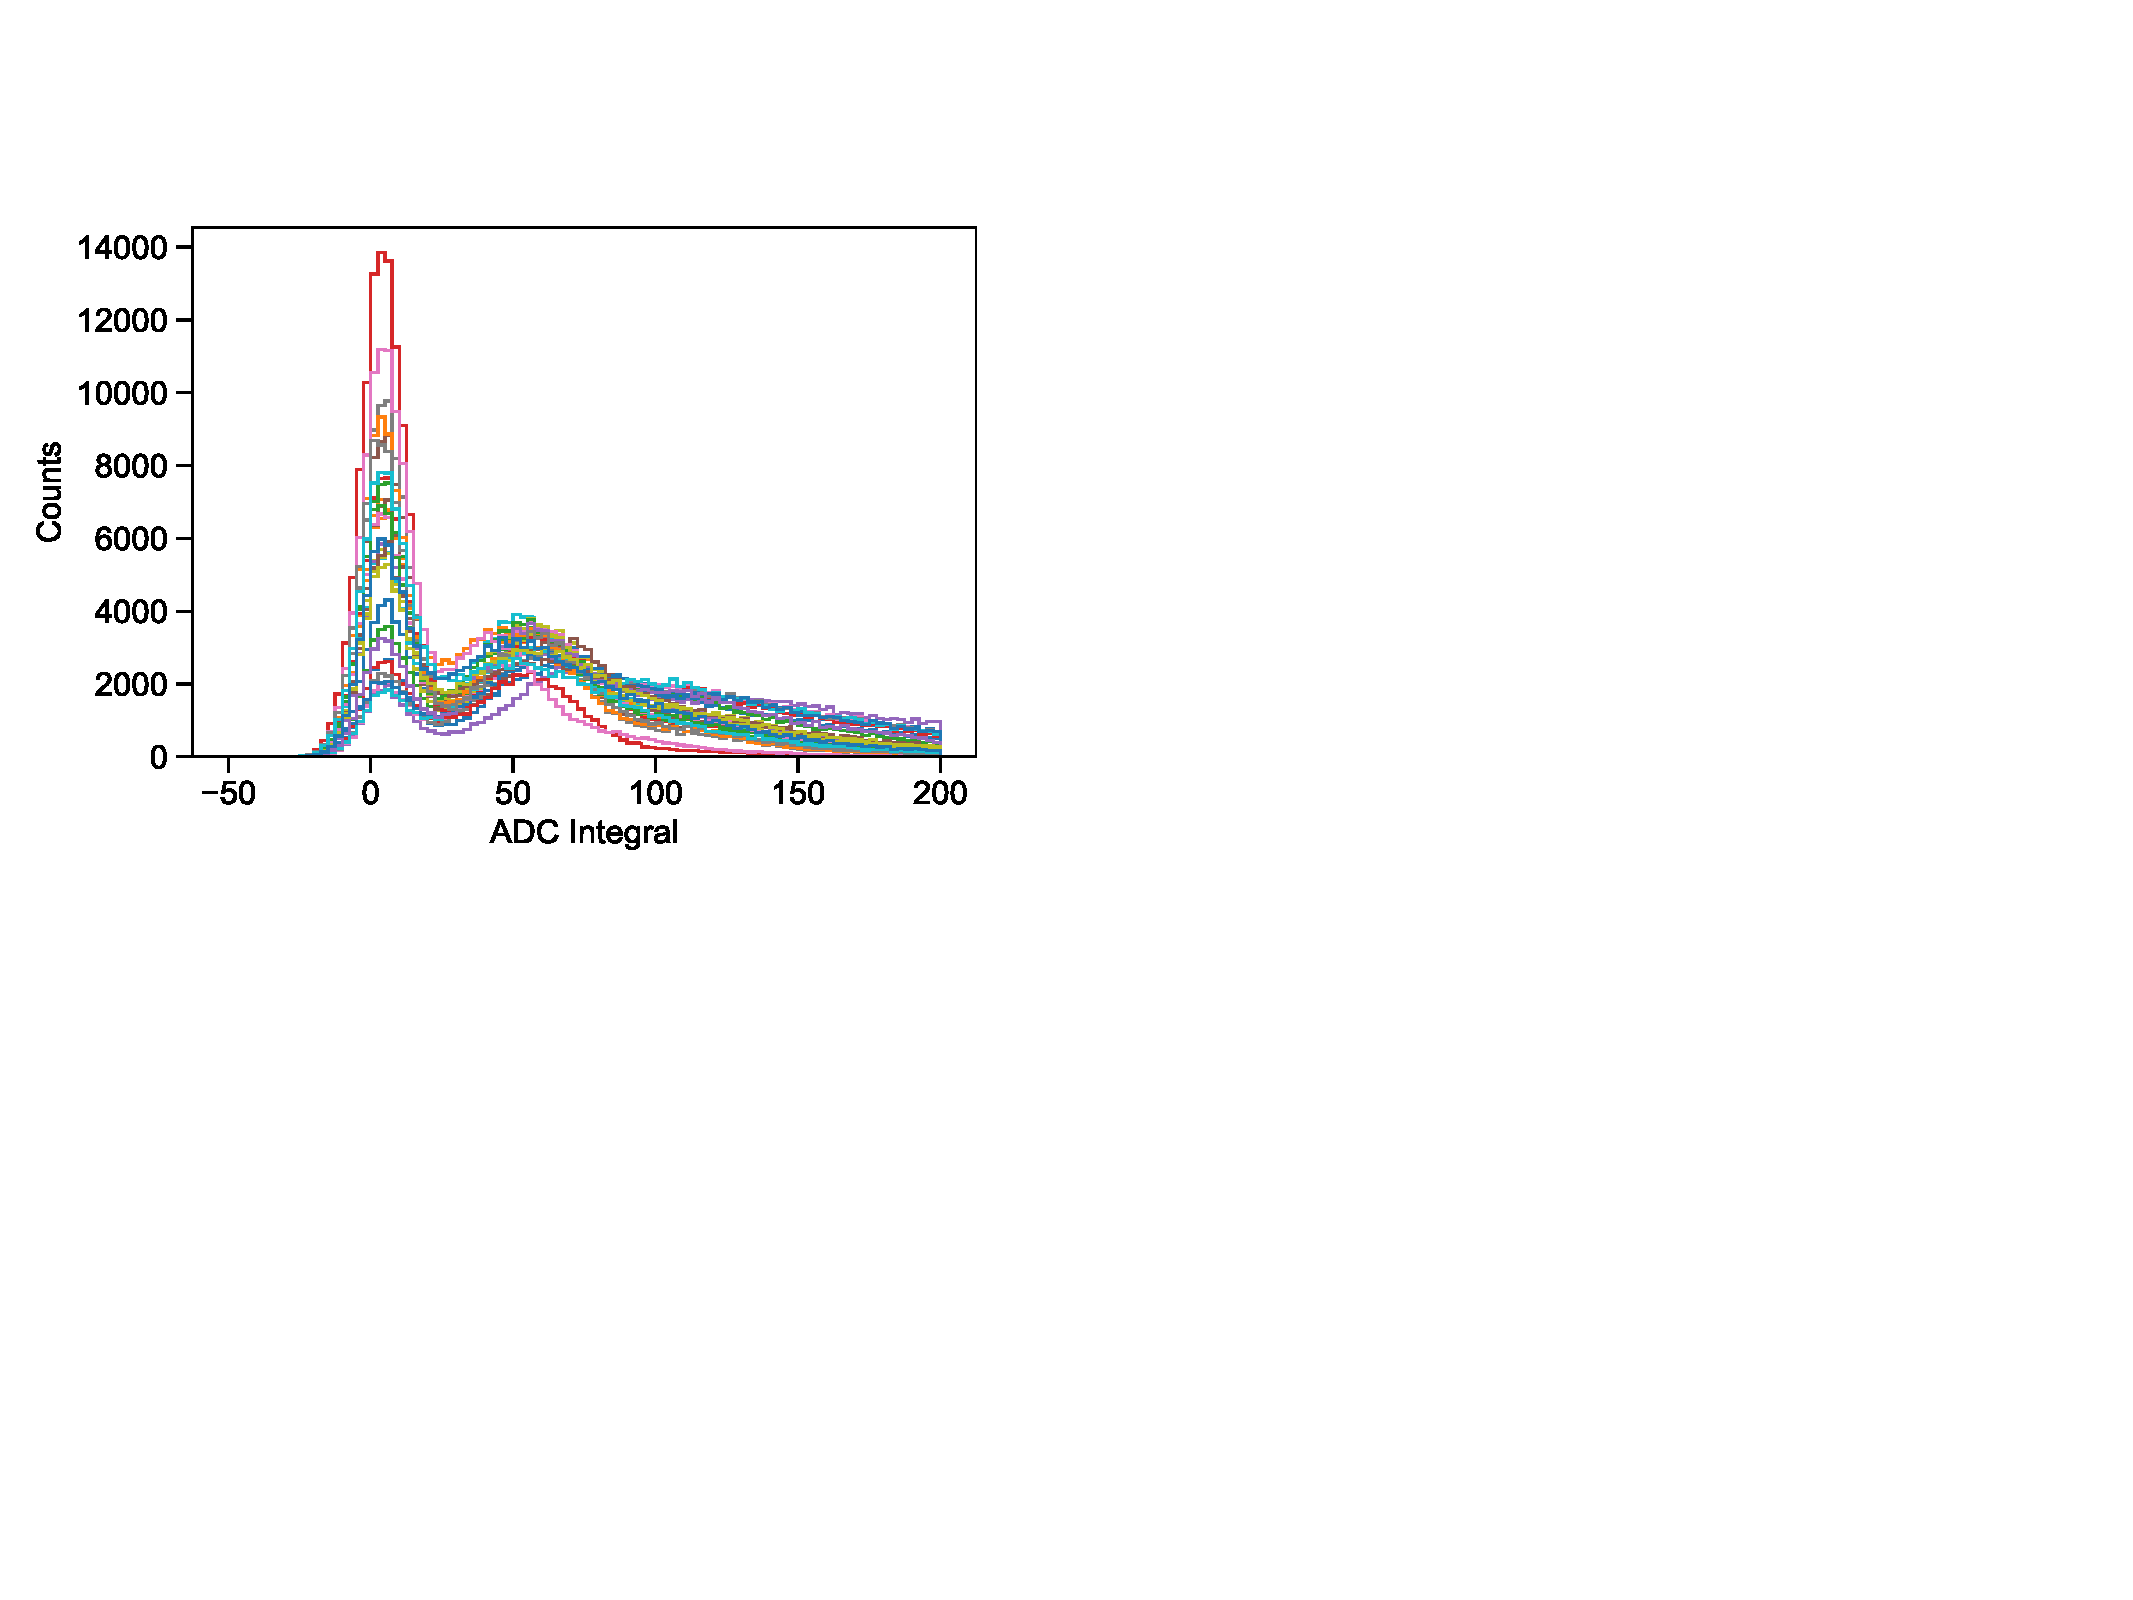
\includegraphics[width=0.48\textwidth]{Figures/SPEADC.pdf}
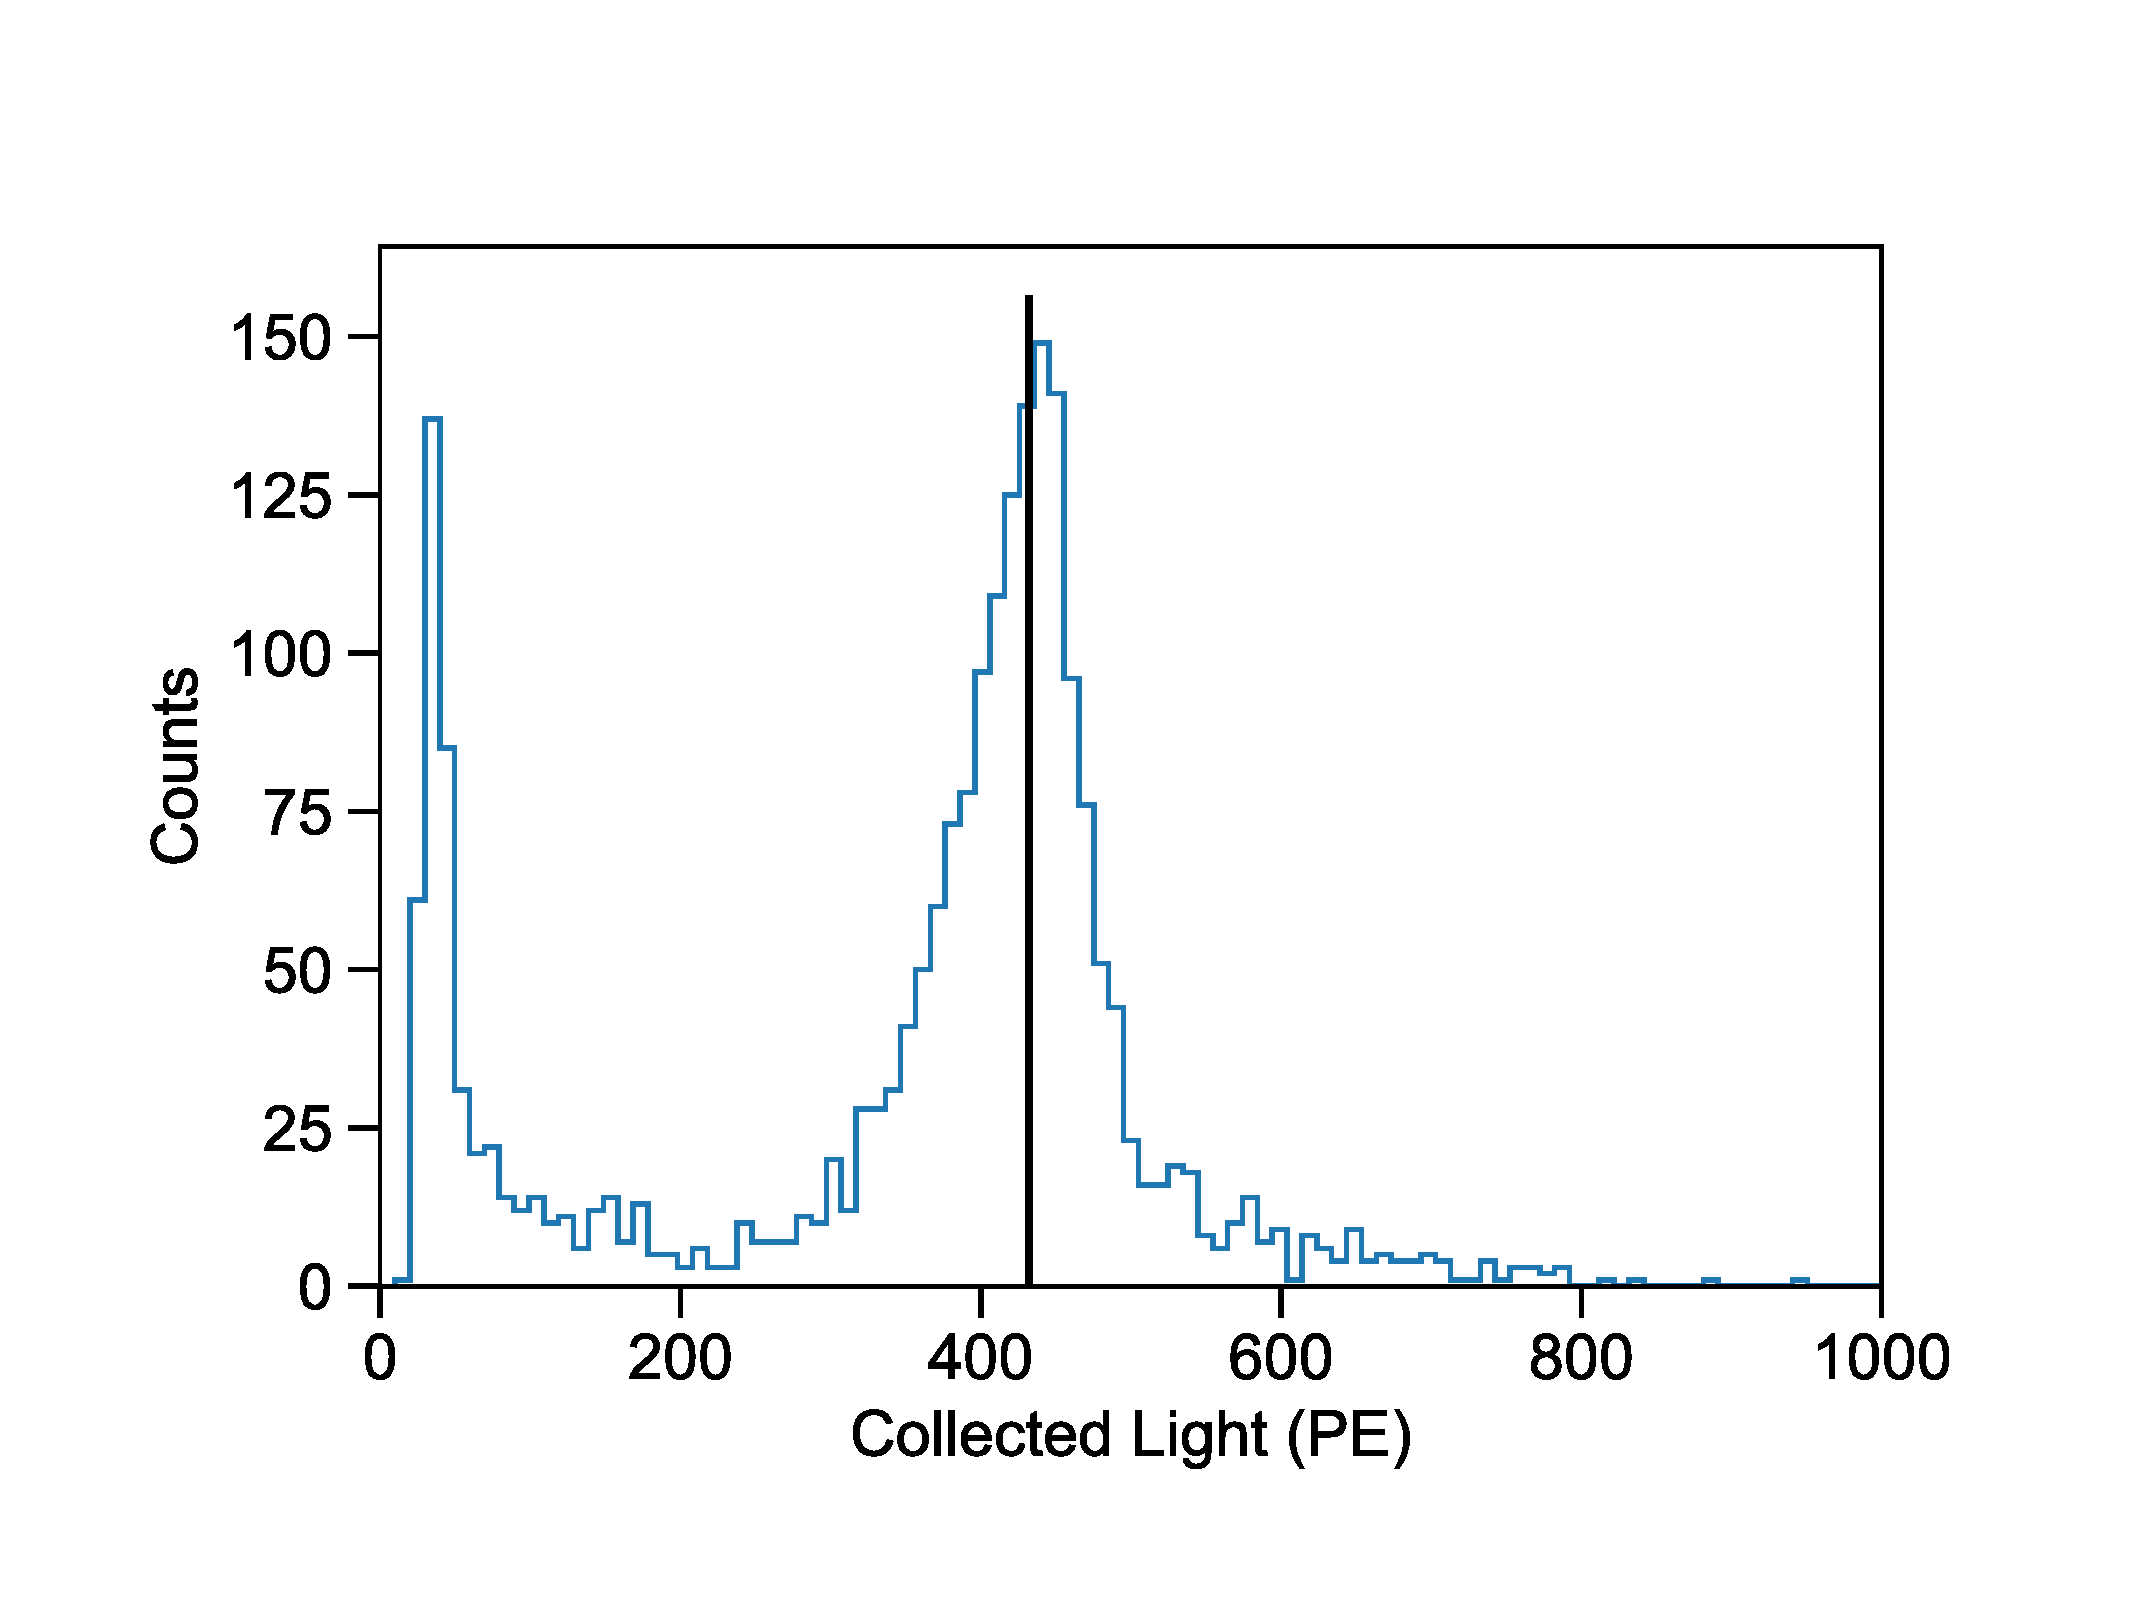
\includegraphics[width=0.48\textwidth]{Figures/SPEnLi.pdf}
\caption[The single PE calibration for photostatistics] {
(Left) The distribution of ADC integrals of single and double PE.
(Right) The distribution of PE amounts of $n$-Li capture with presumed 0.55~MeV, suggesting $\sim$790~PE/MeV photostatistics.
}
\label{fig:SPE}
\end{figure}

\Section{PSD Calibration}

Because of the non-uniform light collection along the $z$-direction, PSD values of events at different position are inconsistent.
Correction of PSD values with respect to $\Delta t$ is made with a simplified function
\begin{equation}
n(dt) = g+d\exp{k \Delta t},
\end{equation}
where $g$, $d$ and $k$ position correction and scale factors.
This function has been demonstrated in the PSD stability tracking.

